\documentclass{article}
\usepackage[utf8]{inputenc}
%\usepackage[english]{babel}
\usepackage[portuguese]{babel}
\usepackage{graphicx}
\usepackage[hidelinks]{hyperref}
\usepackage{amsmath} %lets us use \begin{proof}
%\usepackage[]{amssymb} %gives us the character \varnothing

\title{Universidade Federal de Pernambuco \\
Macroeconomia 1 - Lista 1}
\author{Monitor: Paulo Francisco (paulfsilva7@gmail.com);}
\date{10 de fevereiro de 2023}


\begin{document}
\maketitle %This command prints the title based on information entered above

%Section and subsection automatically number unless you put the asterisk next to them.
\section*{Questão 1}

%Basically, you type whatever text you want and use the $ sign to enter "math mode".
%For fancy calligraphy letters, use \mathcal{}
%Special characters are their own commands

%No Modelo Clássico, suponha que a economia se encontre inicialmente em
%equilíbrio. Discuta os efeitos de um aumento nos impostos sobre a renda do %trabalho. Utilize gráficos para sua explicação e discuta o passo a passo.
\begin{figure}[!tbh]
    \centering
    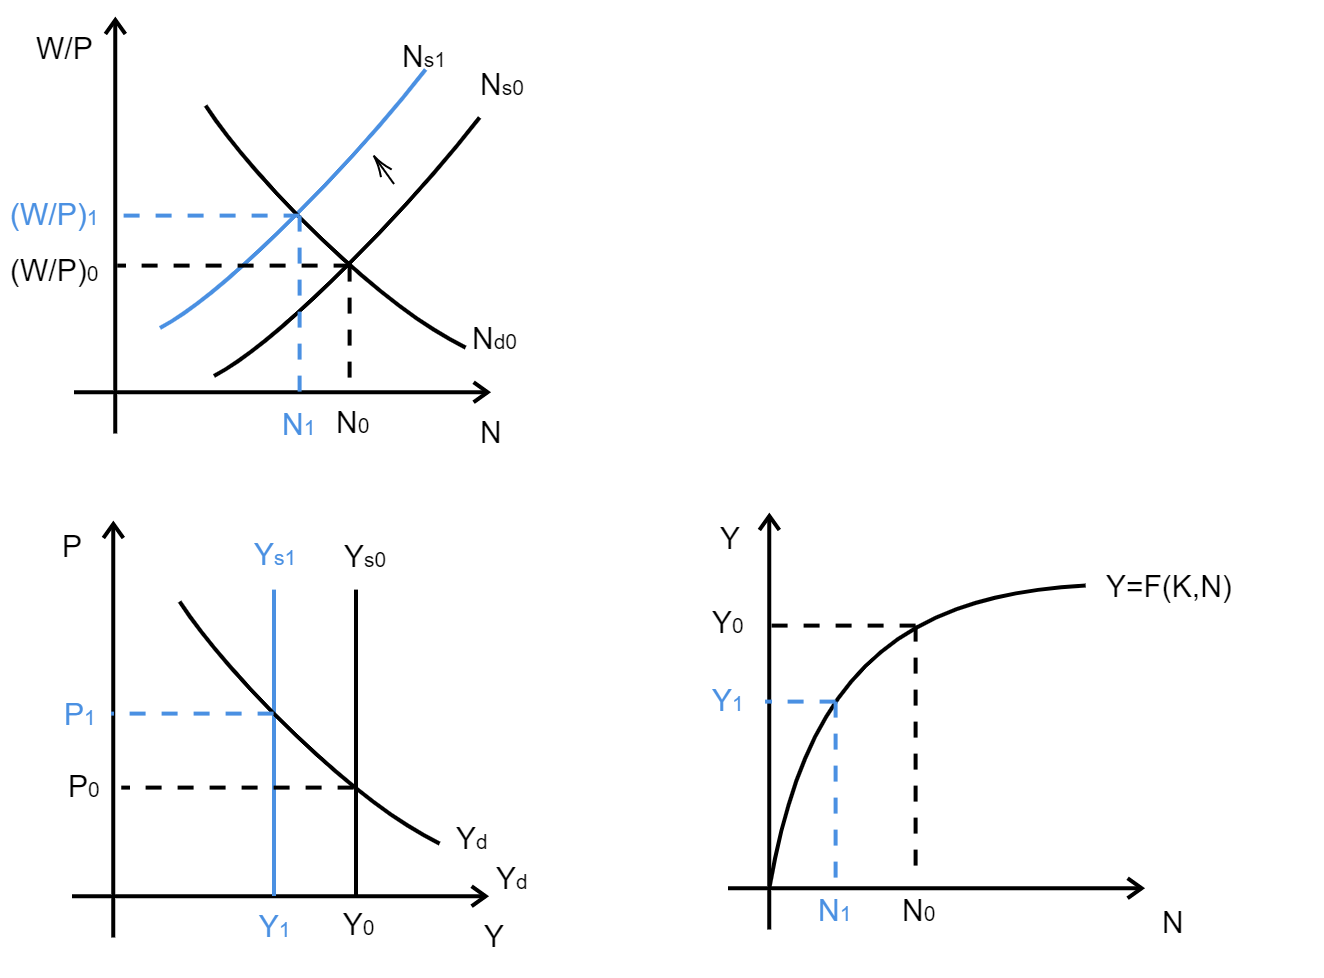
\includegraphics[width=\textwidth]{Grafico - Q1 PNG.png}
    \caption{Resolução no Modelo Clássico}
    \label{fig:GMC1}
\end{figure}

Devido do aumento em $\tau$, a utilidade marginal do lazer cai, ou seja, haverá uma menor oferta de trabalho, deslocando sua da curva para trás.
Com menos trabalho, o nível de produção é menor, retraindo a oferta agregada. Com isso o emprego, o produto e o salário real serão menores em equilíbrio.


\clearpage %Gives us a page break before the next section. Optional.

\section*{Questão 2}

\subsection*{Letra A)}
Dado o enunciado, temos as equações:
$$U(C, L) = ln C + \beta ln L; \quad
N^{s} = 1 - L; \quad
C = (1-\tau)\frac{W}{P}N^s - T;$$
Assim, queremos $\max_{n} U(C,L)$, logo:

\begin{equation}
\frac{\partial U}{\partial N}= \frac{\partial U}{\partial C}\frac{\partial C}{\partial N} + \frac{\partial U}{\partial L}\frac{\partial L}{\partial N}
\end{equation}

\begin{equation}
\frac{\partial U}{\partial N}= \frac{1}{C}(1-\tau)\frac{W}{P} - \beta\frac{1}{L} = 0
\end{equation}

\begin{equation}
\frac{(1-\tau)}{(1-\tau)\frac{W}{P}N-T}\frac{W}{P} = \frac{\beta}{(1-N)}
\end{equation}
\\
Arranjando os termos, têm-se:

\begin{equation}
(1-\tau)(1-N)\frac{W}{P} = \beta[(1-\tau)\frac{W}{P}N-T]
\end{equation}

\begin{equation}
[(1-\tau)\frac{W}{P}] - N(1-\tau)\frac{W}{P} = \beta(1-\tau)\frac{W}{P}N-\beta T
\end{equation}

\begin{equation}
\beta(1-\tau)\frac{W}{P}N + N(1-\tau)\frac{W}{P} = (1-\tau)\frac{W}{P} + \beta T
\end{equation}

\begin{equation}
N\frac{W}{P}[(\beta+1)(1-\tau)] = (1-\tau)\frac{W}{P} + \beta T
\end{equation}
\\
Isolando a oferta de trabalho, N, temos:

\begin{equation}
N = \frac{1}{(\beta+1)} + \frac{\beta T}{\frac{W}{P}(\beta+1)(1-\tau)}
\end{equation}

\clearpage


\subsection*{Letra B)}

Resgatando nossa oferta de trabalho ótima:
\begin{equation}
N = \frac{1}{(\beta+1)} + \frac{\beta T}{\frac{W}{P}(\beta+1)(1-\tau)}
\end{equation}
\\
Calculamos o impacto:

\begin{equation}
\frac{\partial  N}{\partial  \tau} =  \frac{\beta T}{\frac{W}{P}(\beta+1)(1-\tau)^2} > 0
\end{equation}
\\
Nota-se uma relação positiva entre emprego e o imposto sobre a renda do trabalho, de forma que com o aumento em  $\tau$ a oferta de trabalho aumenta.

\clearpage

\subsection*{Letra C)}
Dado o enunciado, temos as equações:
$$U(C, L) = C^\theta + L^{(1-\theta)}; \quad
N^{s} = 1 - L; \quad
C = (1-\tau)\frac{W}{P}N^s - T;$$

Podemos linearizar a função utilidade de forma que temos:
$$ U(C,L) = \theta ln C + (1+\theta)ln L$$

Utilizando novamente a regra da cadeia, e substituindo os termos:
\begin{equation}
\frac{\partial U}{\partial N}= \frac{\partial U}{\partial C}\frac{\partial C}{\partial N} + \frac{\partial U}{\partial L}\frac{\partial L}{\partial N}
\end{equation}

\begin{equation}
\frac{\partial U}{\partial N}= \frac{\theta}{C}(1-\tau)\frac{W}{P} - \frac{(1-\theta)}{L} = 0
\end{equation}

\begin{equation}
 \frac{\theta}{[(1-\tau)\frac{W}{P}N-T]}(1-\tau)\frac{W}{P} = \frac{(1-\theta)}{(1-N)}
\end{equation}

\begin{equation}
 (1-N)\theta(1-\tau)\frac{W}{P} = (1-\theta)[(1-\tau)\frac{W}{P}N-T]
\end{equation}

\begin{equation}
-N\theta(1-\tau)\frac{W}{P} + \theta(1-\tau)\frac{W}{P} = (1-\theta)(1-\tau)\frac{W}{P}N - T(1-\theta)
\end{equation}

\begin{equation}
\theta(1-\tau)\frac{W}{P} + T(1-\theta) = (1-\theta)(1-\tau)\frac{W}{P}N + N\theta(1-\tau)\frac{W}{P}
\end{equation}

\begin{equation}
N(1-\tau)\frac{W}{P}[(1-\theta)+\theta] = \theta(1-\tau)\frac{W}{P} + T(1-\theta)
\end{equation}

\begin{equation}
N = \frac{\theta(1-\tau)\frac{W}{P}}{(1-\tau)\frac{W}{P}[(1-\theta)+\theta]} + \frac{T(1-\theta)}{(1-\tau)\frac{W}{P}[(1-\theta)+\theta]}
\end{equation}

\begin{equation}
N = \theta + \frac{T(1-\theta)}{(1-\tau)\frac{W}{P}}
\end{equation}

\clearpage

\subsection*{Letra D)}
Dado o enunciado, temos as equações: 
$$U(C, L) = \frac{C^{(1-\psi)}}{(1-\psi)} - \gamma \frac{N^{(1-\varphi)}}{(1-\varphi)} \quad
N^{s} = 1 - L; \quad
C = (1-\tau)\frac{W}{P}N^s - T;$$
\\
Podemos realizar uma transformação linear:
$$ U(C,L) = (1-\psi) ln C - ln(1-\psi) - ln \gamma - (1-\varphi) ln N + ln (1-\varphi) $$
\\
Utilizando novamente a regra da cadeia, e substituindo os termos:
\begin{equation}
\frac{\partial U}{\partial N}= \frac{\partial U}{\partial C}\frac{\partial C}{\partial N} + \frac{\partial U}{\partial N}
\end{equation}

\begin{equation}
\frac{\partial U}{\partial N}= \frac{(1-\psi)}{C}(1-\tau)\frac{W}{P} - \frac{(1-\varphi)}{N} = 0
\end{equation}

\begin{equation}
\frac{(1-\psi)}{[(1-\tau)\frac{W}{P}N-T]}(1-\tau)\frac{W}{P} = \frac{(1-\varphi)}{N}
\end{equation}

\begin{equation}
N(1-\psi)(1-\tau)\frac{W}{P} = (1-\varphi)[(1-\tau)\frac{W}{P}N-T]
\end{equation}

\begin{equation}
- N(1-\psi)(1-\tau)\frac{W}{P} + (1-\varphi)(1-\tau)\frac{W}{P}N = T(1-\varphi)
\end{equation}

\begin{equation}
N \frac{W}{P}(1-\tau)[(1-\varphi)-(1-\psi)] = T(1-\varphi)
\end{equation}

\begin{equation}
N = \frac{T(1-\varphi)}{\frac{W}{P}(1-\tau)[(1-\varphi)-(1-\psi)]}
\end{equation}

\clearpage

\section*{Questão 3}
Dados:

$$ C = c_0 + c_1[Y(1-t_y)]$$
$$G=T=t_y Y$$
$$I = A -ai$$
$$\frac{M^{d}}{P} = \bar{l} - il_i + l_y Y$$
$$\frac{M^D}{P}=\frac{M}{P}$$

\subsection*{Letra i)}
Organizando as curvas IS e LM, temos:

\begin{equation}\label{eq:3yi}
Y = c_0 + c_1[Y(1-t_y)] + G + A -ai 
\end{equation}

\begin{equation}\label{eq:3ii}
i = \frac{l_y Y}{l_i} + \frac{\bar{l} - \frac{\bar{M}}{P}}{li}
\end{equation}
\\
Substituindo \eqref{eq:3ii} em \eqref{eq:3yi}:
\begin{equation}
Y = c_0 + c_1(Y(1-t_y)) + G + A -a(\frac{l_y Y}{l_i} + \frac{\bar{l} - \frac{\bar{M}}{P}}{li})
\end{equation}
\\
O objetivo é isolar Y:

\begin{equation}
Y = c_0 + c_1 Y(1-t_y) + G + A -a\frac{l_y Y}{l_i} -a( \frac{\bar{l} - \frac{\bar{M}}{P}}{li})
\end{equation}

\begin{equation}
Y - Y(1-t_y)c_1 + a\frac{l_y Y}{l_i} = c_0 + G + A -a( \frac{\bar{l} - \frac{\bar{M}}{P}}{li})
\end{equation}

\begin{equation}
Y(1 - (1-t_y)c_1 + a\frac{l_y }{l_i}) = c_0+ G + A -a( \frac{\bar{l} - \frac{\bar{M}}{P}}{li})
\end{equation}
\\
Portanto o Y em equilíbrio é:
\begin{equation}\label{eq:3ystari}
Y* =\frac{ c_0 + G + A -a( \frac{\bar{l} - \frac{\bar{M}}{P}}{li})}{(1 - (1-t_y)c_1 + a\frac{l_y }{l_i})}
\end{equation}
\\
Substituindo \eqref{eq:3ystari} em \eqref{eq:3ii}, para encontrar a taxa de juros de equilíbrio:

\begin{equation}
i* = \frac{l_y}{l_i}(\frac{ c_0 + G + A -a( \frac{\bar{l} - \frac{\bar{M}}{P}}{li})}{(1 - (1-t_y)c_1 + a\frac{l_y }{l_i})}) + \frac{\bar{l} - \frac{\bar{M}}{P}}{li}
\end{equation}
\clearpage

\subsection*{Letra ii)}
Tomando Y* como:
\begin{equation}
Y* =\frac{ c_0 + G + A -a( \frac{\bar{l} - \frac{\bar{M}}{P}}{li})}{(1 - (1-t_y)c_1 + a\frac{l_y }{l_i})}
\end{equation}

\begin{equation}
\frac{\partial Y*}{\partial \frac{M}{P}} = \frac{1}{(1 - (1-t_y)c_1 + a\frac{l_y }{l_i})} \frac{a}{l_i} > 0
\end{equation}
\\
Nota-se uma relação positiva entre encaixes reais e o produto, de forma que, uma politica monetária expansionista eleva o produto.
\bigskip
\\
Tomando i* como:
\begin{equation}
i* = \frac{l_y}{l_i}(\frac{ c_0 + G + A -a( \frac{\bar{l} - \frac{M^{d}}{P}}{li})}{(1 - (1-t_y)c_1 + a\frac{l_y }{l_i})}) + \frac{\bar{l} - \frac{\bar{M}}{P}}{li}
\end{equation}

\begin{equation}
\frac{\partial i*}{\partial \frac{\bar{M}}{P}} = \frac{\partial i }{\partial Y }\frac{\partial Y}{\partial \frac{\bar{M}}{P}} + \frac{\partial i}{\partial \frac{M}{P}} 
\end{equation}

\begin{equation}
\frac{\partial i*}{\partial \frac{\bar{M}}{P}} = \frac{l_y}{l_i}\frac{1}{(1 - (1-t_y)c_1 + a\frac{l_y }{l_i})} \frac{a}{l_i} - \frac{1}{l_i}
\end{equation}

\begin{equation}
\frac{\partial i*}{\partial \frac{\bar{M}}{P}} = \frac{1}{l_i} \left[ \frac{l_y a}{(1 - (1-t_y)c_1 + a\frac{l_y }{l_i})} - 1 \right] < 0
\end{equation}
\\
É possível notar dois efeitos: o aumento do produto eleva a taxa de juros, mas o aumento do encaixes reais a reduz, ou seja, depende de qual efeito é maior.
Nota-se uma relação negativa entre oferta de moedas e taxa de juros, ou seja, uma política monetária expansionista levaria a uma redução da taxa de juros, quando o efeito do encaixes reais é maior do que o do produto.
\clearpage

\section*{Questão 4}
Dados:

$$ C = c_0 + c_1(Y - T) $$
$$ I = A - i_r r $$
$$G=20$$
$$ \frac{M}{P} =  \bar{m} + m_1 Y - m_2 i $$
$$M=25, P=5, G=T=20$$

\subsection*{Letra A)}
Organizando as curvas IS e LM:

\begin{equation}\label{eq:4ya}
Y = c_0 + c_1(Y - T) + A - i_r r + G
\end{equation}

\begin{equation}\label{eq:4ia}
i =  \frac{\bar{m}-\frac{M}{P}}{m_2} + \frac{m_1}{m_2} Y
\end{equation}
\\
Substituindo \eqref{eq:4ia} em \eqref{eq:4ya} e isolando Y:

\begin{equation}
Y = c_0 + c_1(Y - T) + A - i_r (\frac{\bar{m}-\frac{M}{P}}{m_2} + \frac{m_1}{m_2} Y) + G
\end{equation}

\begin{equation}
Y = c_0 + c_1Y - c_1 T + A - i_r \frac{\bar{m}-\frac{M}{P}}{m_2} -i_r \frac{m_1}{m_2} Y + G
\end{equation}

\begin{equation}
Y - c_1Y + i_r \frac{m_1}{m_2} Y = c_0 - c_1 T + A - i_r \frac{\bar{m}-\frac{M}{P}}{m_2} + G
\end{equation}

\begin{equation}
Y (1 - c_1 + i_r \frac{m_1}{m_2}) = c_0 - c_1 T + A - i_r \frac{\bar{m}-\frac{M}{P}}{m_2} + G
\end{equation}
\\
Então, o produto de equilíbrio será:
\begin{equation}\label{eq:4ystara}
Y* = [c_0 - c_1 T + A - i_r \frac{\bar{m}-\frac{M}{P}}{m_2} + G] \frac{1}{(1 - c_1 + i_r \frac{m_1}{m_2})}
\end{equation}
\\
Substituindo \eqref{eq:4ystara} em \eqref{eq:4ia}, a tade de juros de equilibrio será:

\begin{equation}
i* =  \frac{\bar{m}-\frac{M}{P}}{m_2} + \frac{m_1}{m_2} [c_0 - c_1 T + A - i_r \frac{\bar{m}-\frac{M}{P}}{m_2} + G] \frac{1}{(1 - c_1 + i_r \frac{m_1}{m_2})}
\end{equation}
\\
Substituindo os parâmetros num software, temos:\\
$Y*= 143.48$; $i*=10.61$; $C* = 113.78$; $I*=9.69$
\clearpage

\subsection*{Letra B)}
Substituindo os parâmetros para a nova simulação, teremos:
$$Y^*= 160.87; i^*=11.65; C^*=111.69; I^*=9.17;$$
\\
Nota-se um aumento do produto, da taxa de juros, mas redução no consumo e investimento, observando então o efeito crowding out.

\subsection*{Letra C)}
Substituindo os parâmetros para a nova simulação, teremos:
$$Y^*= 147.82; i^*=8.87; C^*=117.26; I^*=10.56;$$
\\
Comparando em relação à letra A, nota-se um aumento do produto, consumo e investimento, porém uma redução na taxa de juros.
\clearpage

\section*{Questão 5)}
Dados:
$$C = c_0 + c_1 Y_D - c_2 r$$
$$I = b_0 + b_1 Y_D - b_2 r$$
$$G = g_0$$
$$T = t_0 + t_1 Y$$
$$\frac{M^D}{P}=d_0 + d_1Y - d_2 r$$
$$\frac{M^D}{P}=\frac{\Bar{M}}{P}$$

\section*{Letra A)}

Encontrando a LM:
\begin{equation}\label{eq:5ai}
r=\frac{d_1Y}{d_2}+\frac{d_0}{d_2}-\frac{\bar{M}}{P d_2}
\end{equation}
\\
Organizando produto:
\begin{equation}
Y = c_0 + c_1 Y_D - c_2 r + b_0 + b_1 Y_D - b_2 r + g_0
\end{equation}

\begin{equation}
Y = c_0 + c_1 (Y- t_0 - t_1 Y) - c_2 r + b_0 + b_1 (Y-t_0 - t_1 Y) - b_2 r + g_0
\end{equation}

\begin{equation}
Y = c_0 + c_1 Y- c_1 t_0 - c_1t_1 Y - c_2 r + b_0 + b_1 Y - b_1 t_0 - b_1 t_1 Y - b_2 r + g_0
\end{equation}

\begin{equation}\label{eq:5ay}
Y = c_0 +  Y(c_1-c_1t_1+b_1- b_1 t_1) - c_1 t_0 - r(c_2+b_2) + b_0 - b_1 t_0 + g_0
\end{equation}
\\
Substituindo \eqref{eq:5ai} em \eqref{eq:5ay}:
\begin{equation}
Y = c_0 +  Y(c_1-c_1t_1+b_1- b_1 t_1) - c_1 t_0 - (\frac{d_1Y}{d_2}+\frac{d_0}{d_2}-\frac{\bar{M}}{P d_2})(c_2+b_2) + b_0 - b_1 t_0 + g_0
\end{equation}
\\
Isolando Y, tem-se:
\begin{equation}
Y = c_0 +  Y(c_1-c_1t_1+b_1- b_1 t_1-\frac{d_1}{d_2}(c_2+b_2)) - c_1 t_0 - (\frac{d_0}{d_2}-\frac{\bar{M}}{P d_2})(c_2+b_2) + b_0 - b_1 t_0 + g_0
\end{equation}

\begin{equation}
Y[1-(c_1+b_1)(1-t_1)+\frac{d_1}{d_2}(c_2+b_2)]= c_0 - (c_1+b_1)t_0 - (\frac{d_0}{d_2}-\frac{\bar{M}}{P d_2})(c_2+b_2) + b_0+ g_0
\end{equation}
\\
Logo o produto de equilíbrio será:
\begin{equation}\label{eq:5ays}
Y^*=\frac{c_0 - (c_1+b_1)t_0 - (\frac{d_0}{d_2}-\frac{\bar{M}}{P d_2})(c_2+b_2) + b_0+ g_0}{[1-(c_1+b_1)(1-t_1)+\frac{d_1}{d_2}(c_2+b_2)]}
\end{equation}
\\
Substituindo \eqref{eq:5ays} em \eqref{eq:5ai}, temos a taxa de juros em equilíbrio:
\begin{equation}\label{eq:5ais}
r^*=\frac{d_1}{d_2}(\frac{c_0 - (c_1+b_1)t_0 - (\frac{d_0}{d_2}-\frac{\bar{M}}{P d_2})(c_2+b_2) + b_0+ g_0}{[1-(c_1+b_1)(1-t_1)+\frac{d_1}{d_2}(c_2+b_2)]})+\frac{d_0}{d_2}-\frac{M^D}{P d_2}
\end{equation}

\subsection*{Letra B)}
\subsubsection*{Para o produto:}
\begin{equation}
\frac{\partial Y}{\partial g_0} = \frac{1}{[1-(c_1+b_1)(1-t_1)+\frac{d_1}{d_2}(c_2+b_2)]} > 0
\end{equation}
\\
Nota-se uma relação positiva entre os gastos do governo e o produto, de forma que quanto maior o gasto maior o produto.

\subsubsection*{Para a taxa de juros:}
\begin{equation}
\frac{\partial r^*}{\partial g_0} = \frac{d_1}{d_2} \frac{1}{[1-(c_1+b_1)(1-t_1)+\frac{d_1}{d_2}(c_2+b_2)]} > 0
\end{equation}
\\
Nota-se uma relação positiva entre os gastos do governo e a taxa de juros, de forma que quanto maior o gasto maior a taxa de juros.

\subsubsection*{Para o consumo:}
\begin{equation}
\frac{\partial C}{\partial g_0} = \frac{\partial C}{\partial Y}\frac{\partial Y}{g_0} + \frac{\partial C}{\partial r}\frac{\partial r}{\partial g_0}
\end{equation}

\begin{equation}
\frac{\partial C}{\partial g_0} = \frac{c_1(1-t_1)- c_2 d_1}{d_2[1-(c_1+b_1)(1-t_1)+\frac{d_1}{d_2}(c_2+b_2)]}
\end{equation}
\\
É ambíguo, depende de qual efeito é maior.\\
Considerando o efeito da renda agregada é maior do que o efeito da taxa de juros nota-se uma relação positiva entre os gastos do governo e o consumo, de forma que quanto maior o gasto maior o consumo.
\bigskip

\subsubsection*{Para o investimento:}
\begin{equation}
\frac{\partial I}{\partial g_0} = \frac{\partial I}{\partial Y}\frac{\partial Y}{g_0} + \frac{\partial I}{\partial r}\frac{\partial r}{\partial g_0}
\end{equation}

\begin{equation}
\frac{\partial I}{\partial g_0} = \frac{b_1(1-t_1)-d_1}{d_2[1-(c_1+b_1)(1-t_1)+\frac{d_1}{d_2}(c_2+b_2)]}
\end{equation}
\\
É ambíguo; depende de qual efeito é maior.\\
Considerando o efeito da renda agregada é maior do que o efeito da taxa de juros nota-se uma relação positiva entre os gastos do governo e o investimento, de forma que quanto maior o gasto maior o investimento.

\subsection*{Letra C)}
\begin{equation}
\frac{\partial I}{\partial g_0} = \frac{\partial I}{\partial Y}\frac{\partial Y}{g_0} + \frac{\partial I}{\partial r}\frac{\partial r}{\partial g_0}
\end{equation}
Um aumento nos gastos do governo aumenta a taxa de juros, $\frac{\partial r^*}{\partial g_0} > 0$, o que desestimula o investimento, $\frac{\partial I}{\partial r^*} < 0$, ou seja, com o aumento da taxa de juros, há uma redução nos investimentos, portanto nota-se o efeito crowding out.

\clearpage

\section*{Questão 6)}
Dados:
$$C = \bar{C} + c_y (Y - \bar{T}) - c_r r^{e}; \hspace{0.5cm} I = \bar{I} + i_y (Y - \bar{T}) - i_r r^{e}+ z;$$
$$ G = \bar{G}; \hspace{0.5cm} T = \bar{T}; \hspace{0.5cm} 
i = \bar{i}; \hspace{0.5cm} r^{e} = r + s; \hspace{0.5cm} r=i-\pi^{e};$$

%\begin{equation}
%Y_n =\frac{\bar{C} - \bar{T}(c_y+i_y ) + \bar{I} - (i_r+c_r)(r+s)+ z + %G}{[1-(c_y+i_y)]}
%\end{equation}

\subsection*{Letra A)}
Analiticamente, teremos: 
$$
\frac{\partial Y }{\partial s } < 0; \hspace{0.8cm}
\frac{\partial C }{\partial s } < 0; \hspace{0.8cm}
\frac{\partial I }{\partial s } < 0;$$
Há uma relação negativa com o prêmio de risco, de forma que com a queda do prêmio de risco, o consumo, o investimento e o produto aumentam, deslocando a curva IS para a direita. Dado que o Banco Central determina o juros, e, querendo manter o mesmo nível de produto anterior, este pode aumentar a taxa nominal de juros, deslocando a curva LM para cima, e reduzindo o consumo, investimento e produto.

\begin{figure}[!tbh]
    \centering
    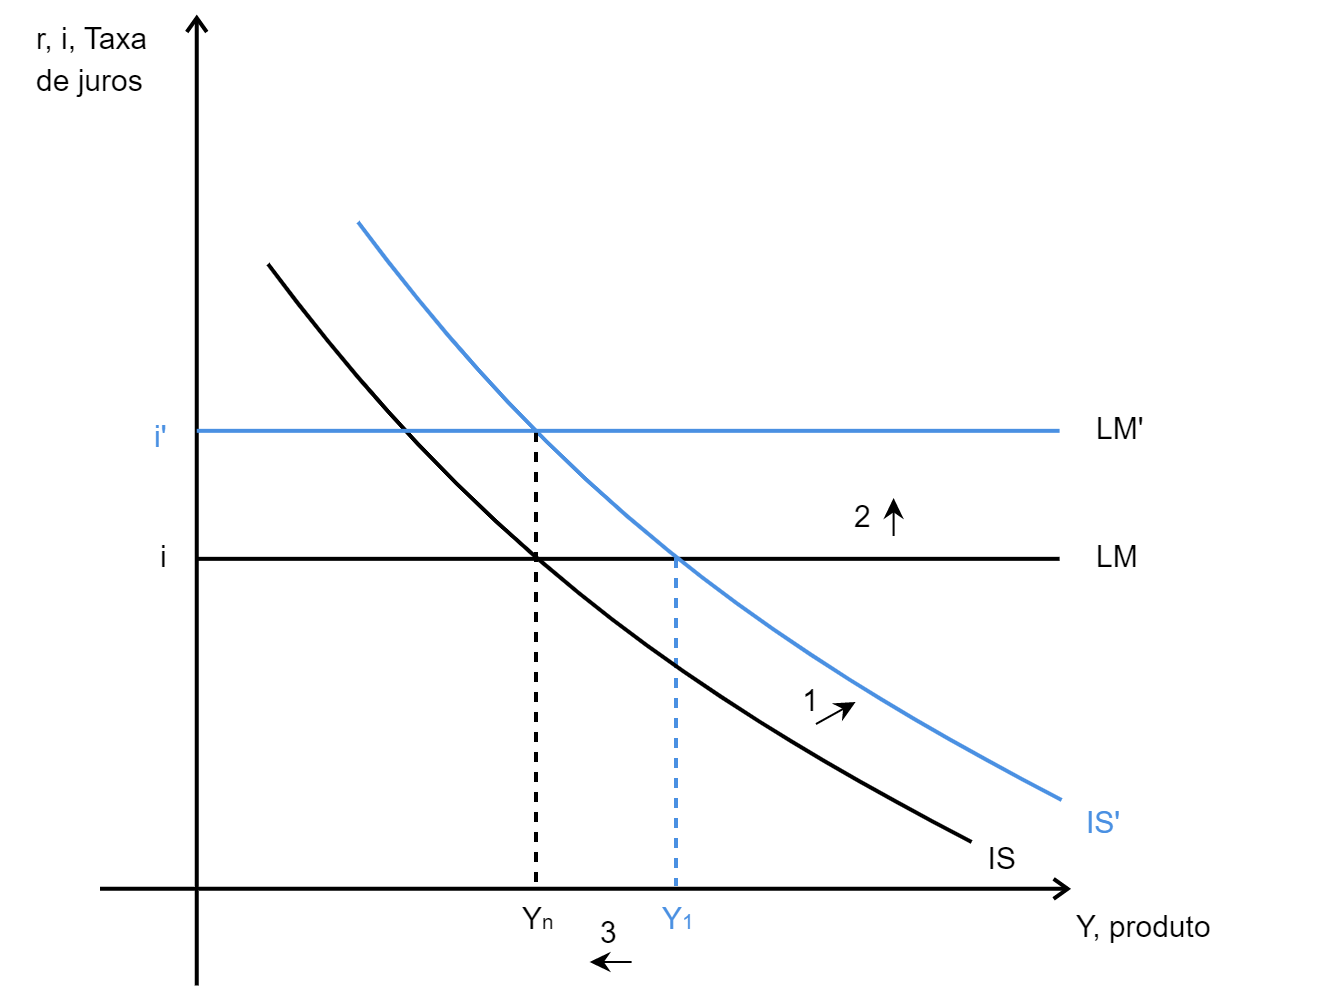
\includegraphics[width=\textwidth]{Grafico - Q6A PNG.png}
    \caption{IS-LM: Choque no prêmio de risco}
\end{figure}

\clearpage

\subsection*{Letra B)}

\begin{figure}[!tbh]
    \centering
    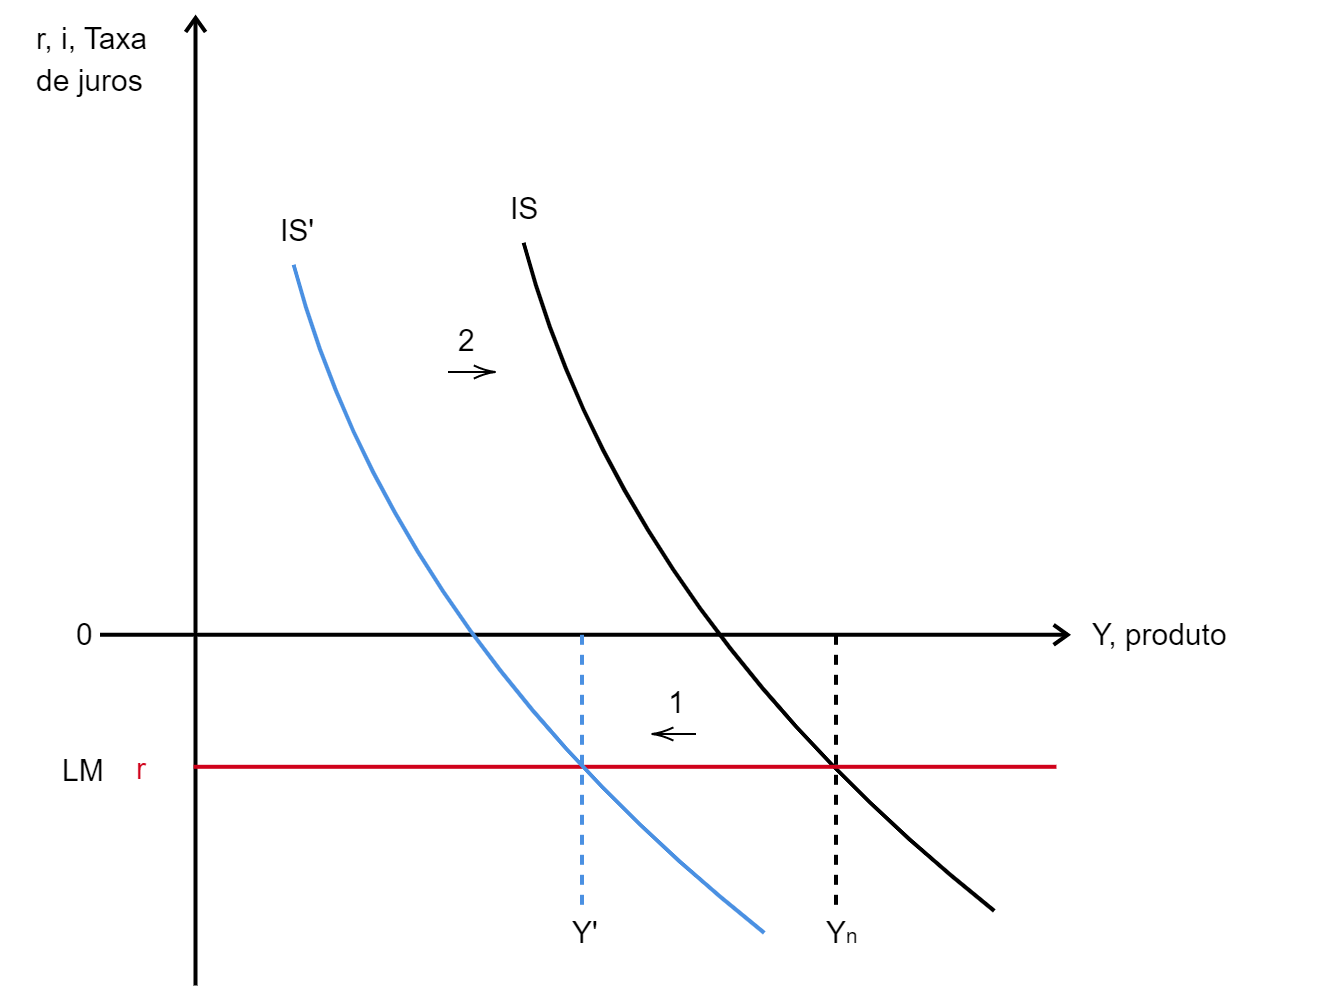
\includegraphics[width=\textwidth]{Grafico - Q6B PNG.png}
    \caption{IS-LM: Choque sanitário negativo}
\end{figure}

O choque negativo desloca a curva IS para esquerda, porém, com a taxa de juros nominal zero, a política monetária se torna inefetiva. Logo, para restaurar o equilíbrio inicial o governo pode fazer uma expansão fiscal, $\Delta G > 0$, de forma que o produto aumentaria, levando a curva IS de volta à inicial.

\clearpage

\section*{Questão 7)}

\begin{equation}
Y = [c_1 + e]Y_D +  I_0 - I_1 r + g_0
\end{equation}

\begin{equation}
Y = [c_1 + e](Y- t_0 -t_1 Y) +  I_0 - I_1 r + g_0
\end{equation}

\begin{equation}
Y = [c_1 + e](1-t_1)Y - [C_1 +e]t_0 +  I_0 - I_1 r + g_0
\end{equation}

\begin{equation}
Y [1 - (c_1 + e)(1-t_1)] =  I_0 - I_1 r + g_0 - [C_1 +e]t_0
\end{equation}

\begin{equation}
Y = \frac{ I_0 - I_1 r + g_0 - (cru_1 +e)t_0}{[1 - (c_1 + e)(1-t_1)]}
\end{equation}

\subsection*{Letra A)}

\begin{figure}[!tbh]
    \centering
    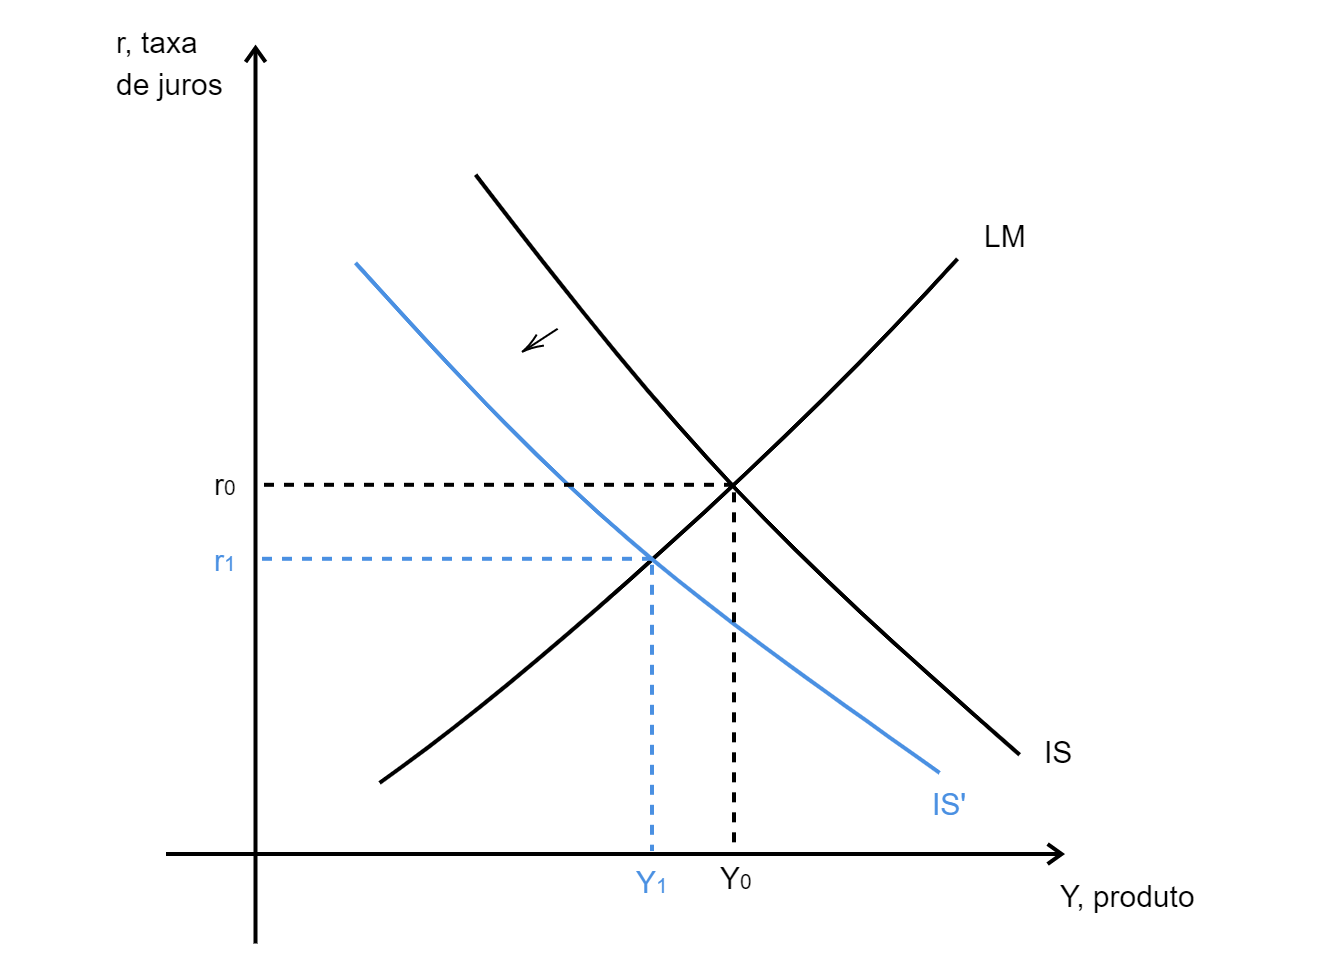
\includegraphics[width=\textwidth]{Grafico - Q7A PNG.png}
    \caption{IS-LM: Choque de expectativas negativas}
\end{figure}

Na ocorrência de um pessimismo nota-se que o consumo e produto agregado caem.
Indicando portanto um novo equilíbrio, com menor produto e taxa de juros quando comparado a situação inicial.

\clearpage

\subsection*{Letra B)}

\begin{figure}[!tbh]
    \centering
    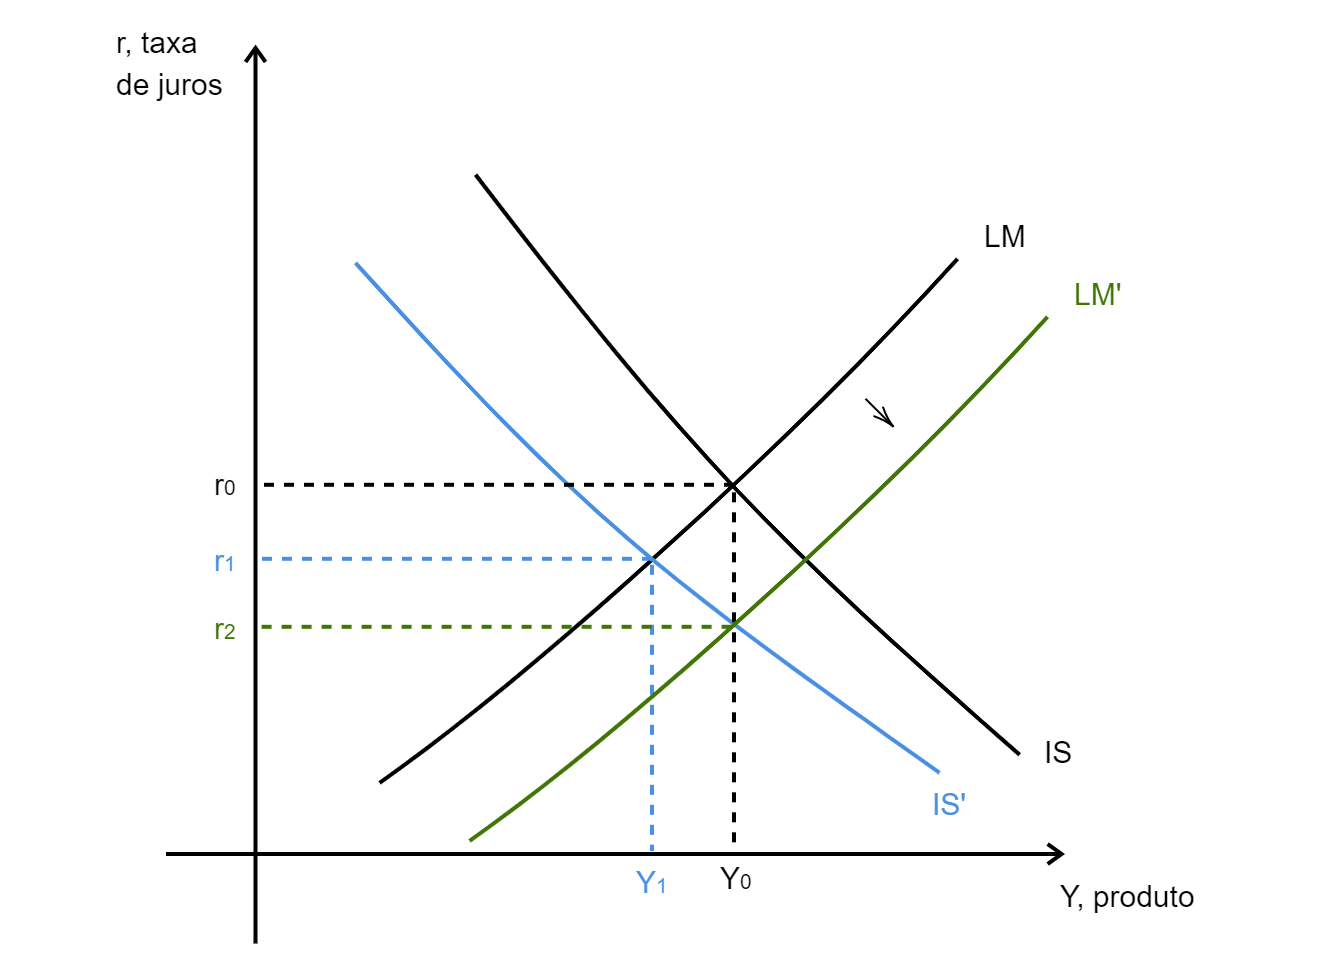
\includegraphics[width=\textwidth]{Grafico - Q7B PNG.png}
    \caption{IS-LM: Politica Monetária Expansionista}
\end{figure}

A politica monetária desloca a curva LM para a direita, podendo restaurar o equilíbrio inicial, expandindo o produto e reduzindo a taxa de juros.

\clearpage

\subsection*{Letra C)}

\begin{figure}[!tbh]
    \centering
    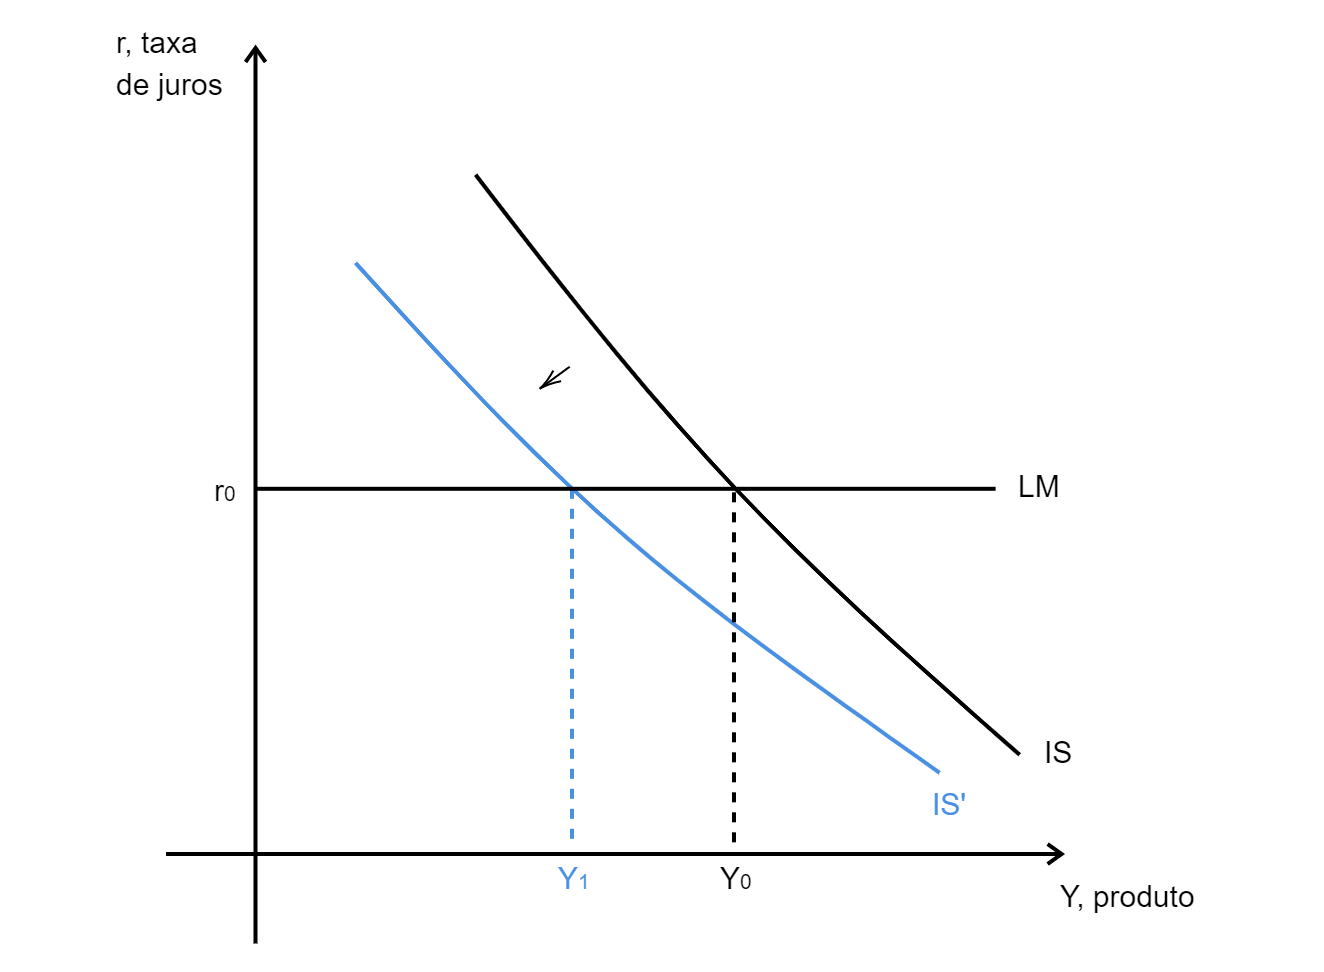
\includegraphics[width=\textwidth]{Grafico - Q7C PNG.png}
    \caption{IS-LM: Choque de expectativas negativas}
\end{figure}

Dado que o Banco Central determina a taxa de juros, a taxa de juros permanece fixa, porém, há uma queda no produto agregado.

\clearpage

\subsection*{Letra D)}

\begin{figure}[!tbh]
    \centering
    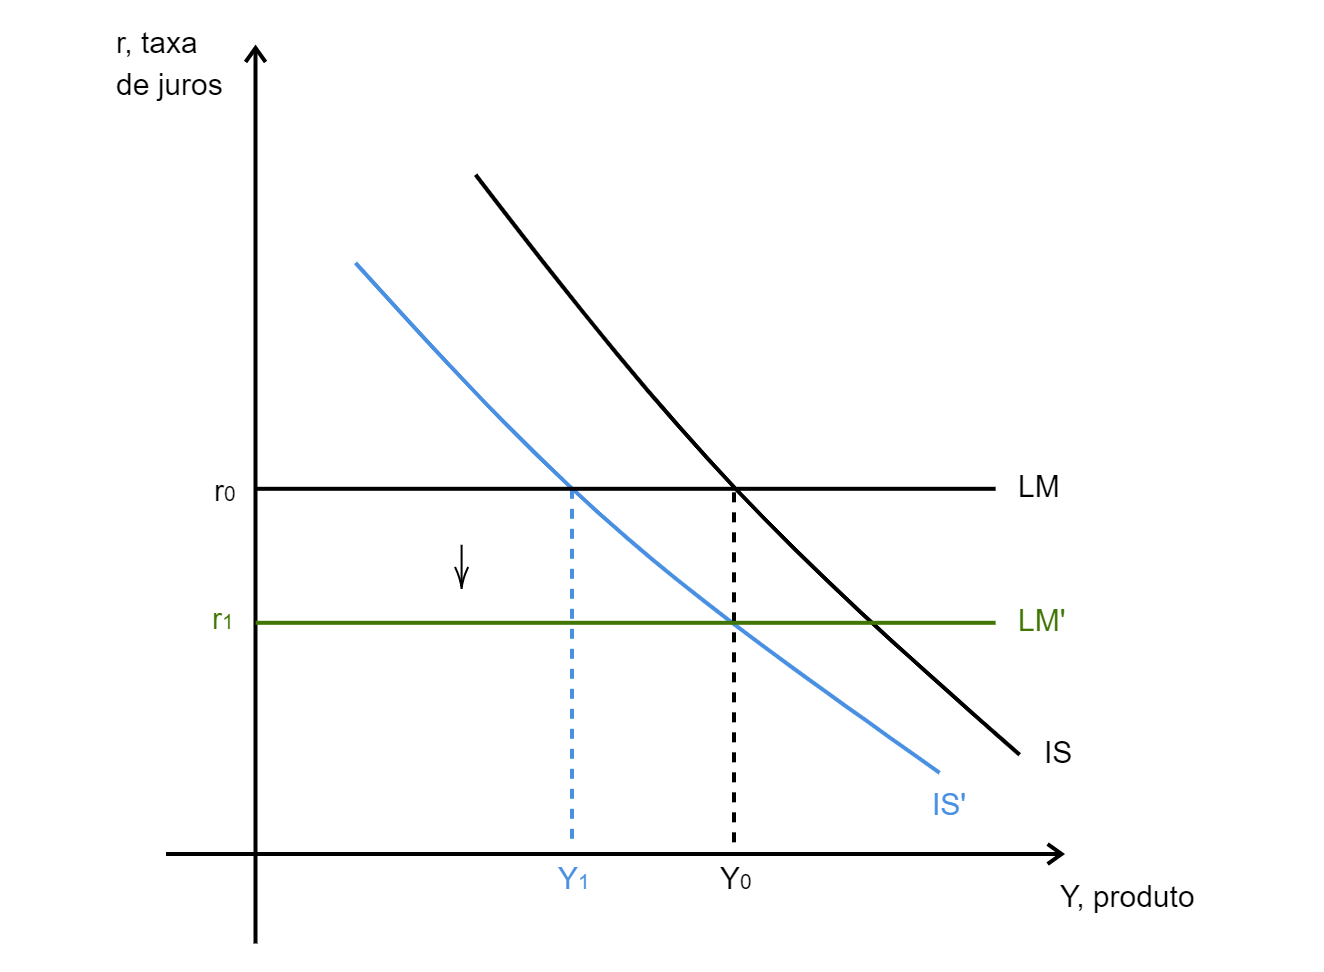
\includegraphics[width=\textwidth]{Grafico - Q7D PNG.png}
    \caption{IS-LM: Politica Monetária Expansionista}
\end{figure}

Com a politica monetária expansionista o Banco Central reduz a taxa de juros, incentivando o aumento do produto até restaurar o equilíbrio inicial. Resultando em um maior produto e menor taxa de juros.

\clearpage

\subsection*{Letra E)}

\begin{figure}[!tbh]
    \centering
    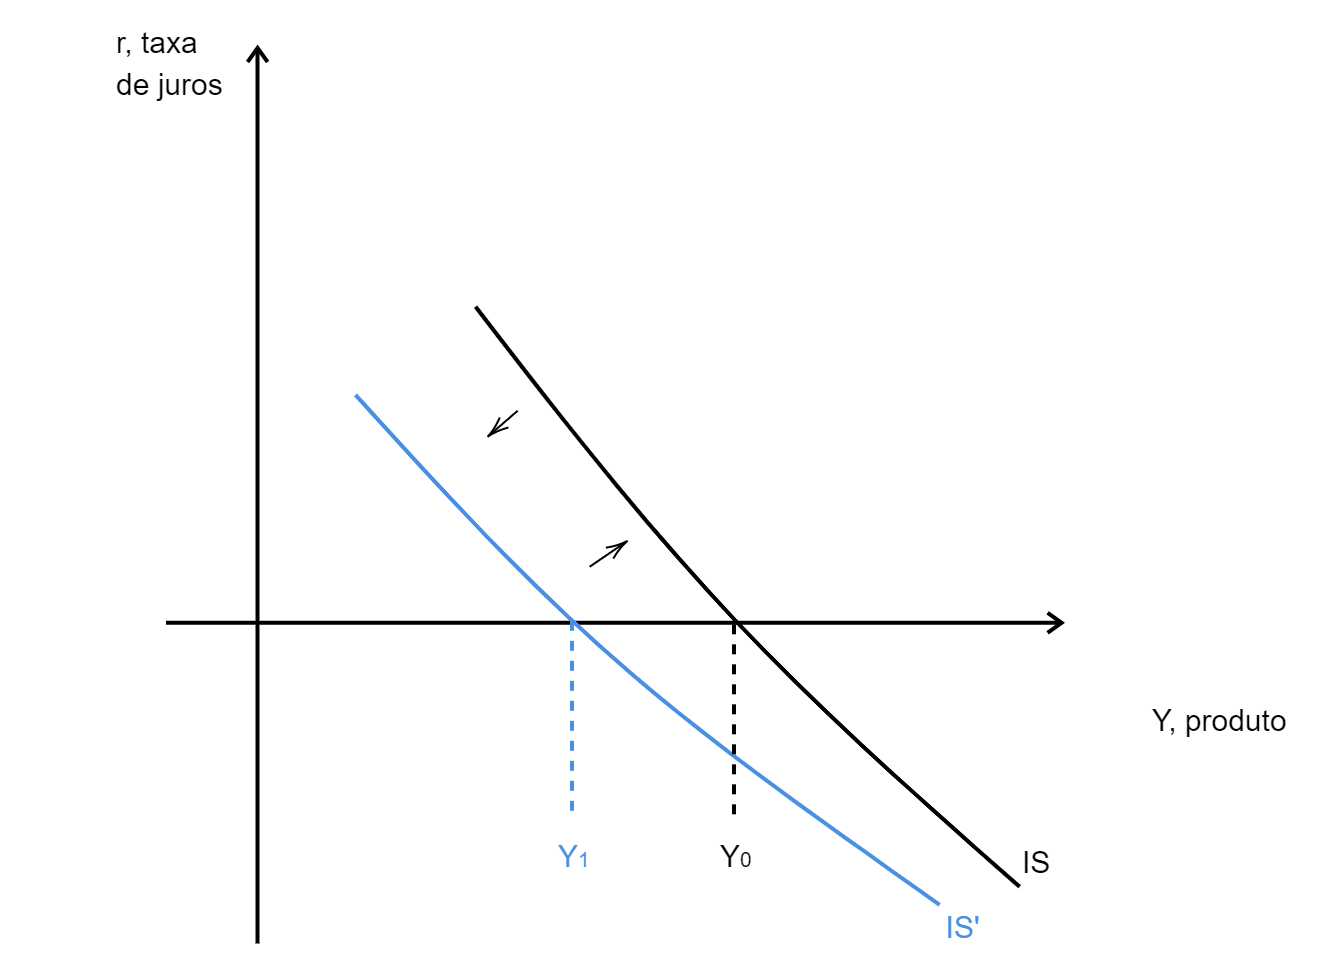
\includegraphics[width=\textwidth]{Grafico - Q7E PNG.png}
    \caption{IS-LM: Armadilha da liquidez}
\end{figure}

Com a taxa de juros nomial igual a zero, ou seja, situação lower bound, a política monetária é inefetiva, direcionando esforços então a política fiscal expansionista, $\Delta G > 0$ por exemplo, de forma que a curva IS se desloca para a direita podendo restaurar o equilíbrio inicial.

\end{document}